\chapter{Mathematical Background}\label{chap:math}

\section{State-space representation of a control system}

State-space representation of a system is a way to model a
physical system by putting the entire system in terms of a set of
first-order differential equations of state variables
$(x_{1},x_{2},\ldots,x_{n})$.  These first-order different
equations can be written out as,

\begin{eqnarray*}
\dot {x}_{1}&=&a_{11}x_{1}+a_{12}x_{2}+\cdots+a_{1n}x_{n}+b_{11}u\\
\dot {x}_{2}&=&a_{21}x_{1}+a_{22}x_{2}+\cdots+a_{1n}x_{n}+b_{21}u\\
\vdots&\\
\dot {x}_{n}&=&a_{n1}x_{1}+a_{n2}x_{2}+\cdots+a_{1n}x_{n}+b_{n1}u\\
\end{eqnarray*}

\noindent where $\dot x=dx/dt$.  This set of differential equation
can be written in the following matrix form:

\begin{displaymath}
\frac{d}{dt}\overbrace{\left[ \begin{array}{c}
                    x_{1}\\
                    x_{2}\\
                    \vdots\\
                    x_{n}
                    \end{array}\right]}^{\textbf{x}\in\mathbb{R}^{n\times1}}=
            \overbrace{\left[\begin{array}{ccc}
                    a_{11}&a_{12}\cdots&a_{1n}\\
                    a_{21}&a_{22}\cdots&a_{2n}\\
                    \vdots\\
                    a_{n1}&a_{n2}\cdots&a_{nn}\\
                    \end{array}\right]}^{\textbf{A}\in\mathbb{R}^{n\times n}}
            \left[ \begin{array}{c}
                    x_{1}\\
                    x_{2}\\
                    \vdots\\
                    x_{n}
                    \end{array}\right]+
            \overbrace{\left[ \begin{array}{c}
                                b_{1}\\
                                b_{2}\\
                                \vdots\\
                                b_{n}
                                \end{array}\right]}^{\textbf{b}\in\mathbb{R}^{n\times1}}u
\end{displaymath}

\medskip The column vector of state variables, \textbf{x}, is called
the state vector.  Since we will be dealing with finite
dimensional systems, the matrices \textbf {A} and \textbf {b} are
constants. The state-space representation can be written in a more
compact form as the state differential equation,

\begin{equation}
\mathbf {\dot x}=\mathbf{Ax}+\mathbf{b}u. \label{eq:statedeq}
\end{equation}

\noindent The outputs of such system can be represented in the
output equation,

\begin{equation}
\mathbf {y}=\mathbf{c^{t}x}+\mathbf{D}u, \label{eq:output}
\end{equation}

\noindent where \textbf{y} is the set of output signals expressed
in column vector form and \textbf{c} $\in\mathbb{R}^{n\times1}$ is
a column vector that varies depending the desired output.

\medskip We will now use the spring-mass system shown in
Figure~\ref{fig:springMass} to illustrate how one could convert a
system from a single higher order differential equation into
state-space representation.  The differential equation governing
the system is,

\begin{displaymath}
m\ddot {x} +d\dot{x} +kx=u,
\end{displaymath}


\begin{figure}
\centering
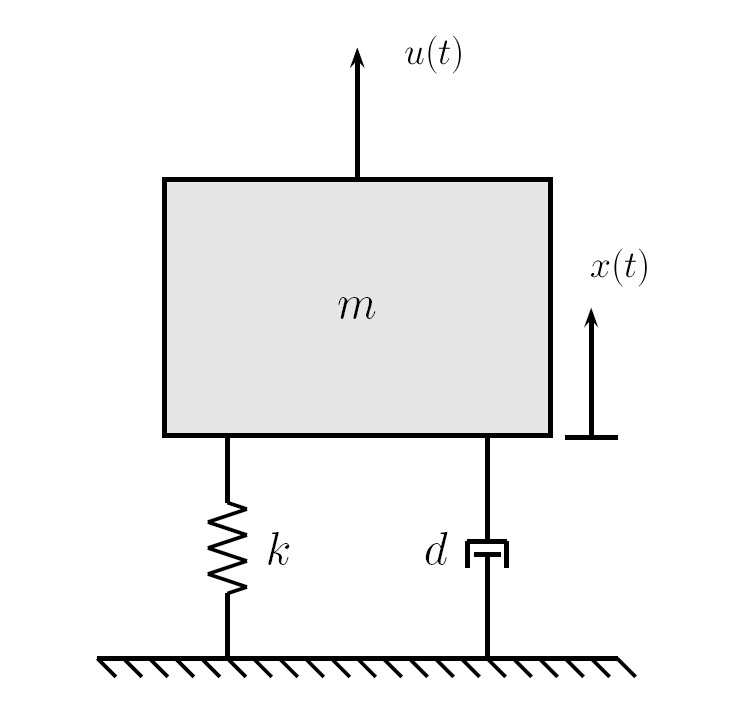
\includegraphics[width=0.7\textwidth]{pix/massSpring.jpg} 
\caption{Mass-Spring-Damper System with input $u(t)$.}
\label{fig:springMass}
\end{figure}

\noindent where u(t) denotes the input force.  First, let us
define $x_{1}=x$ and $x_{2}=\dot {x}$.  The governing equation can
now be written as

\begin{eqnarray*}
\dot x_{1}= \dot x&=&x_{2}\\
\dot x_{2}= \ddot x&=&-\frac{k}{m}x-\frac{d}{m}\dot x+\frac{1}{m}u
=-\frac{k}{m}x_{1}-\frac{d}{m}x_{2}+\frac{1}{m}u
\end{eqnarray*}

\noindent Hence, we can now write the system in the matrix/vector
form as

\begin{eqnarray*}
         \left[\begin{array}{c}\dot x_{1}\\ \dot x_{2}\end{array}\right]&=&\left[\begin{array}{cc} 0&1\\-\frac{k}{m}&-\frac{d}{m}\\\end{array}
        \right]\left[\begin{array}{c} x_{1}\\ x_{2}\end{array}\right]+\left[\begin{array}{c} 0\\\frac{1}{m} \end{array}\right] u.\\
\end{eqnarray*}

\noindent For this system to be in the form of
equation~\ref{eq:statedeq}, we should define

\begin{displaymath}A=\left[\begin{array}{cc}
                    0&1\\
                    -\frac{k}{m}&-\frac{d}{m}\\
                    \end{array}\right], b=\left[
                    \begin{array}{c}
                    0\\\frac{1}{m}
                    \end{array}\right].
\end{displaymath}

\medskip Suppose the desired output of the system is the
displacement of the mass.  We need to have the output to be
$y=x=x_{1}$ and in matrix form we have
\begin{displaymath}
y=\left[\begin{array}{cc}1&0\end{array}\right]\left[\begin{array}{c}x_{1}\\x_{2}\end{array}\right]
\end{displaymath}

\noindent To follow the format of equation~\ref{eq:output}, we
define
\begin{displaymath}
c^{t}=\left[\begin{array}{cc}1&0\end{array}\right], D=[0]
\end{displaymath}

\medskip Now we change the desired output of the system from the displacement to the velocity of the mass.  \textbf{A} and \textbf{b} of the system
will remain the same, but now we need to have the output to be
$y=\dot x=x_{2}$ and in matrix form we have
\begin{displaymath}
y=\left[\begin{array}{cc}0&1\end{array}\right]\left[\begin{array}{c}x_{1}\\x_{2}\end{array}\right]
\end{displaymath}

\noindent To follow the format of equation~\ref{eq:output}, we
define
\begin{displaymath}
c^{t}=\left[\begin{array}{cc}0&1\end{array}\right], D=[0]
\end{displaymath}

\section{Stability of control systems}

Most of you would be familiar with the idea that a system,
$\Sigma\mathbf=({A,b,c^{t},D})$ with the transfer function,

\begin{displaymath}
T_{\Sigma}(s)=\frac{N(s)}{D(s)},
\end{displaymath}

\noindent is BIBO stable if and only if D(s) has roots only in the
negative half-plane.

Another way to find out if a system is is table is by looking at
its impulse response.  We shall define the impulse response of a
given system in state-space form to be,

\begin{displaymath}
h_{\Sigma}= \left\{
\begin{array}{cc}c^{t}e^{At}b, &t\geq0\\0,&otherwise.\end{array}\right.
\end{displaymath}

\noindent With this definition in mind, there exist a theorem that
states that:

\begin{quote}

Let $\Sigma\mathbf=({A,b,c^{t},D})$ be a SISO linear system and
define $\tilde{\Sigma}\mathbf=({A,b,c^{t},0_{1}})$. $\Sigma$ is
BIBO stable if and only if $\lim_{t\rightarrow\infty}|
h_{\tilde{\Sigma}}(t)|=0$.
\end{quote}

It is not difficult too see how these two ways of looking at
stability relate to each other.  The transfer function is a
function in the Laplace domain and if there was a root of D(s) in
$\mathbb{C}_{+}$, the inverse Laplace function, the impulse
response, would have an exponential function with positive
exponents.  The exponential part of the impulse response would
blow up as $t\rightarrow\infty$.  On the other hand, if all the
roots of the transfer function were in $\mathbb{C}_{-}$, the
impulse response would have exponential functions with negative
exponents. Such function would die out to zero as
$t\rightarrow\infty$.


\section{Performance Specifications}
The following is a list of definition needed for Lab 7.

\begin{itemize}
\item\emph {Steady-state value}
\\The final value of the response.
\item\emph {Rise time}
\\The time elapsed up to the instant at which the response
reaches the steady-state value for the first time.
\item\emph
{Overshoot}
\\The maximum amount by which the response exceeds the
steady-state value.
\item\emph {Settling time (or
$\epsilon$-settling time)}
\\The time needed such that the response enters a specified band,
$\pm\epsilon$, without leaving again.
\item\emph {System types}
\\Let $k\geq 0$. A signal $r$ defined on [0,$\infty$) is of
\emph{type k} if $r(t)=Ct^{k}$ for some $C>0$.  A BIBO stable SISO
linear system (N,D) is of \emph{type k} if
$\lim_{t\rightarrow\infty}(r(t)-y(t))$ exists and is nonzero for
every controller output $(r(t),y(t))$ with $r(t)$ of type k.
\item\emph {Error}
\\The error for a controller output $(r(t),y(t))$ is
$e(t)=r(t)-y(t)$.
\item\emph {Steady-state error}
\\The steady-state error for a controller output $(r(t),y(t))$ is
$\lim_{t\rightarrow\infty}(r(t)-y(t))$.
\end{itemize}

Except for the definition of system types, all of the above
definition should be self-explanatory.  The following proposition
should be helpful on determining the system type of a given SISO
linear system.

\begin{quote}
Let $\Sigma$=(N,D) be a BIBO stable SISO linear system in
input/output form.  The following are equivalent:

\begin{enumerate}
\item $\Sigma$=(N,D) is of type k. \item
$\lim_{t\rightarrow\infty}(r(t)-y(t))$  exists and is nonzero for
some controller output (r(t),y(t)) with r(t) of type k. \item
$\lim_{s\rightarrow\infty} \frac{1}{s^{k}}(1-T_{\Sigma}(s))$
exists and is nonzero.
\end{enumerate}
\end{quote}

\section{Nyquist Criterion}

A proof of how Nyquist plots and the Nyquist Criterion work
requires the understanding of Cauchy's theorem and contours
mapping in complex variable theory.  Fortunately, it is not
necessary to understand the proof in order to use Nyquist plots as
a tool in control engineering.

\subsection{Interconnected bounded-input, bounded-output stability (IBIBO stability)}
The idea of IBIBO stability is similar to BIBO stability.  A
system shown in Figure~\ref{fig:closedLoop}

\begin{figure}[htbp]
    \centering
    \begin{picture}(230,75)
    \put(0,50){\(\hat\theta_{d}(s)\)}
    \put(20,53){\vector(1,0){15}}
    \put(40,53){\circle{7}}
    \put(45,53){\vector(1,0){20}}
    \put(68,37){\framebox(35,33){\normalsize \(R_{C}(s)\)}}%-50 in width
    \put(105,53){\vector(1,0){40}}
    \put(147,37){\framebox(35,33){\normalsize \(R_{P}(s)\)}}
    \put(185,53){\vector(1,0){30}}
    \put(217,50){\(\hat\theta(s)\)}
    \put(201,53){\line(0,-1){45}}
    \put(201,8){\line(-1,0){161}}
    \put(40,8){\vector(0,1){40}}
    \put(30,48){\line (1,0) {4}}
    \end{picture}
    \caption{Feedback system with disturbance}\label{fig:closedLoop}
\end{figure}

\noindent has the closed-loop transfer function of

\begin{displaymath}
T(s)= \frac{R_{C}(s)R_{P}(s)}{1+R_{C}(s)R_{P}(s)}.
\end{displaymath}

For a system to be IBIBO stable, the poles of the closed-loop
transfer function must all be in $\mathbb{C}_{-}$.

\subsection{The Nyquist criterion for closed-loop stability}

Let $R_{C}$ and $R_{P}$ be rational function with
$R_{L}=R_{C}R_{P}$ proper.  Let $n_{p}$ be the number of poles of
$R_{L}$ in $\mathbb{C}_{+}$.  The interconnected SISO linear
system represented by block diagram Figure~\ref{fig:closedLoop} is
IBIBO stable if and only if
\begin{enumerate}
\item there are non cancellations of poles and zeros in
$\mathbb{C}_{+}$ between $R_{C}$ and $R_{P}$; \item
$\lim_{s\rightarrow\infty}R_{L}(s)\neq -1$; \item the number of
counterclockwise encirclements of the the point -1+\emph{i}0 in
the complex plane is equal $n_{p}$.
\end{enumerate}

The first two part of the above theorem should be self
explanatory.  The last part of the theorem simply means that if
the open-loop transfer function, $R_{L}$, has n poles in
$\mathbb{C}_{+}$, then the corresponding Nyquist contour of
$R_{L}$ should have n counterclockwise encirclements of the point
-1+\emph{i}0.

\subsection{Examples}

For the following examples, we'll assume that the first two
conditions of the Nyquist criterion are true.

\begin{enumerate}
\item $R_{L}(s)=R_{C}(s)R_{P}(s)=\frac{1}{s-3}$,
$T_{L}=\frac{1}{s-2}$

Looking at the closed-loop transfer function, we know that the
system is not IBIBO stable.  A look at the Nyquist plot
(Figure~\ref{fig:unstable}) would confirm that result because
while $R_{L}$ has a pole in $\mathbb{C}_{+}$, there is no
counterclockwise encirclement of the point -1+\emph{i}0.

\item $R_{L}(s)=R_{C}(s)R_{P}(s)=\frac{s+7}{(s+3)(s-2)}$,
$T_{L}=\frac{s+7}{s^{2}+2s+1}$

From the closed-loop transfer function, the system is clearly
IBIBO stable.  Since $R_{L}$ has one pole in $\mathbb{C}_{-}$ and
the Nyquist plot (Figure~\ref{fig:stable}) shows there is one
counterclockwise encirclement of the point -1+\emph{i}0, the
result from the Nyquist plot agrees with the result from analyzing
the pole of the closed-loop transfer function.


\begin{figure}
\centering
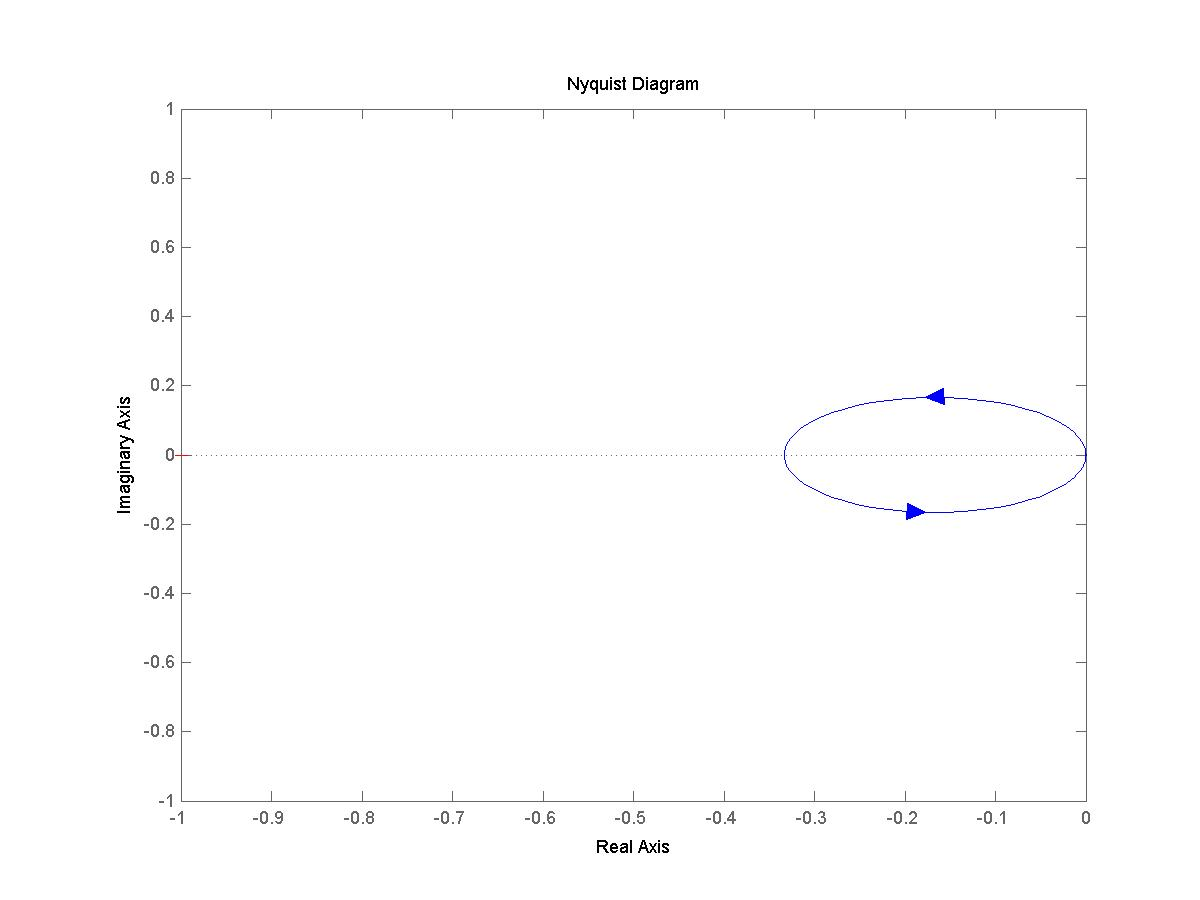
\includegraphics[width=0.7\textwidth]{pix/matheg1.jpg} 
\caption{Nyquist plot when $R_{L}(s)=R_{C}(s)R_{P}(s)=\frac{1}{s-3}$.}
\label{fig:unstable}
\end{figure}

\begin{figure}
\centering
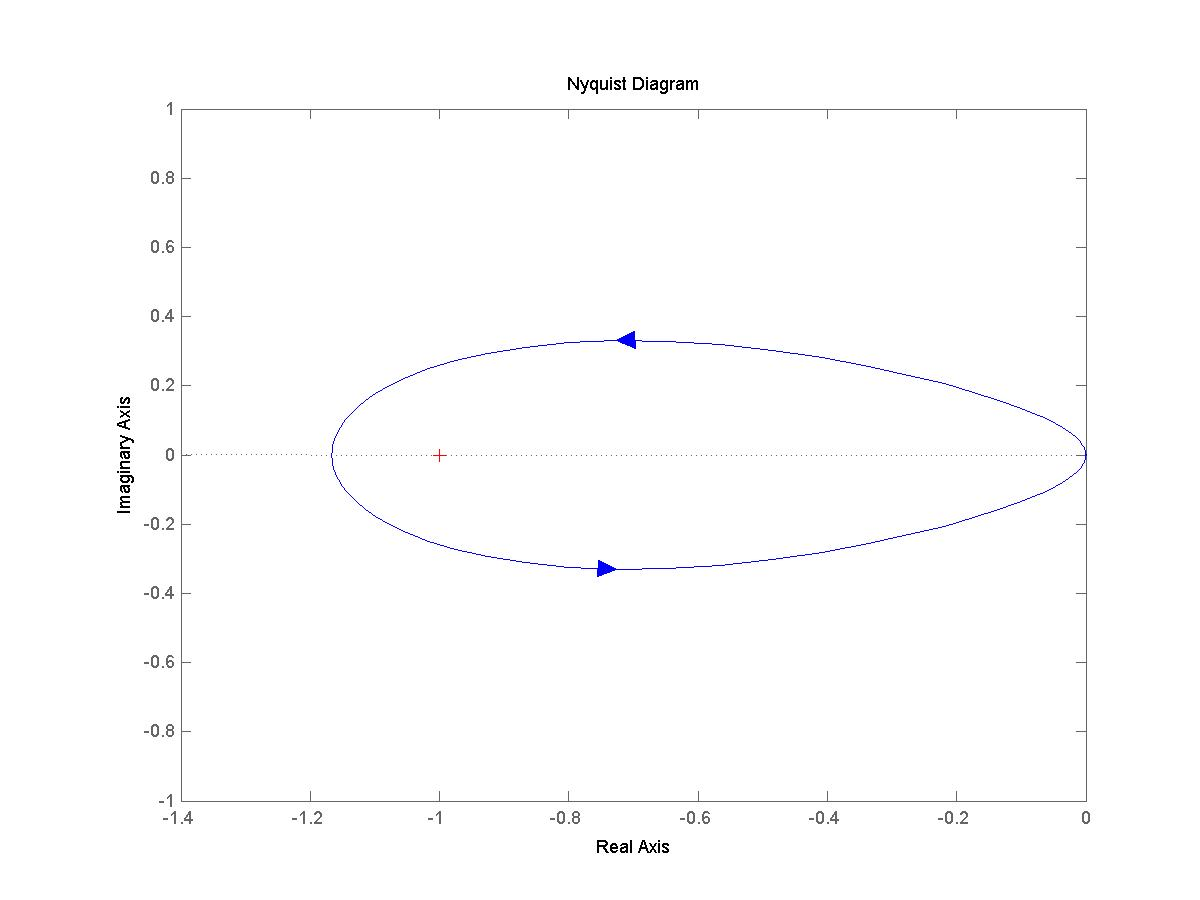
\includegraphics[width=0.7\textwidth]{pix/matheg2.jpg}
\caption{Nyquist plot when $R_{L}(s)=R_{C}(s)R_{P}(s)=\frac{s+7}{(s+3)(s-2)}$.} 
\label{fig:stable}
\end{figure}

\end{enumerate}

%%% Local Variables: 
%%% mode: latex
%%% TeX-master: "lab-manual"
%%% End: 
